\begin{figure*}[t]
\centering
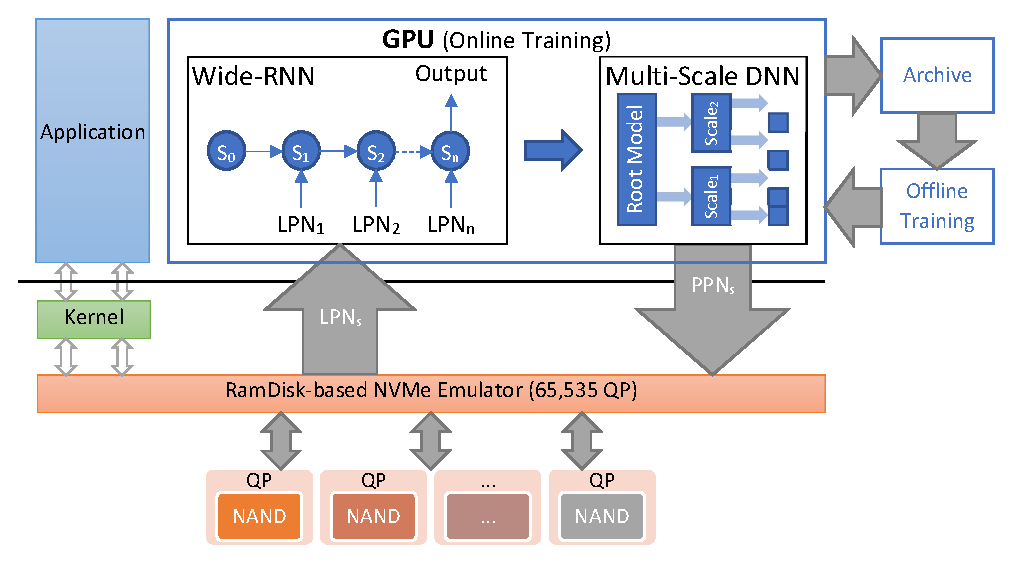
\includegraphics[width=0.8\textwidth]{fig/emulator.eps}
\caption{Prototype of Learned Storage based on the NVMe SSD Emulator. (LPN: Logical page number. PPN: Physical page number.)}
\label{fig:emulator_architecture}

\end{figure*}\section{Implementation and Evaluation}

We employ our open-sourced SSD emulator~\cite{zhou2018cpftl} to implement
a prototype system of learned log-structured storage architecture.
% To develop a working system within a reasonable time frame,
Most of existing ML frameworks expose their programming interfaces through
high-level programming languages, such as Python and Java.
This also allows for ease of tuning of ML algorithms and execution parameters.
However, current main stream storage systems are developed in C/C++.
A great portion of them runs at kernel device driver level or even device firmware level.
It is an intimidating job of developing ML algorithms at either device driver or firmware level.
More importantly, it could be infeasible to conduct sensitivity
test and tune different ML algorithms at low level architectures.

We develop a working system on top of our open-sourced SSD emulator~\cite{zhou2018cpftl},
which reserves a large physical DRAM space to mimic the external storage devices.
Our in-house GPU cluster serves as the host, among which node is configured with 2 Intel Xeon E5,
2.2 GHz 12-core, 128GB DRAM and four NVIDA GeForce GTZ Titan XP Graphics card, 12 GB GDDR5X cards. 
We offload most of the low-level functionalities
at either kernel space or device firmware to the user space.
In the user space, we are free to choose any high-level ML libraries
and programming languages for quick implementation.
Once the prototype system is tuned well and validated mature,
we can move forward to re-implement the functions by the low-level languages.

Figure~\ref{fig:emulator_architecture} shows the architecture of SSD emulator
based learned storage prototype.
At kernel space, SSD emulator reserves large amounts of contiguous memory
at boot time as the emulated flash memory.
% The NVMe protocol with 65K queues is built to directly handle the logic page number of logic block request (LBA in brief).
Since current machine learning support at kernel space is very limited,
we implement page-level Flash Translation Layer (i.e., FTL in brief) at user space.
For efficiency, we employ a validated version of our in-house page-level FTL
protocol to perform address translation between logical page number and physical page number.

\subsection{Experimal Results}

To gauge the effectiveness and efficiency of our TAC,
we conducted a comprehensive set of experiments,
and collected results about the cache hit ratio of I/O accesses
from our working SSD Emulator based prototype.
We implemented the FTL module using different cache and prefetching algorithms.
Regarding the learned I/O prefetcher module,
we first implemented our TAC algorithm to split mixed workloads.
Afterwards, we employ the LSTM model to predict the future I/Os.
We used both synthetic and real-world traces and divided traces into training part and testing part.

\begin{figure*}[t]
  \centering
  \begin{subfigure}[b]{0.45\textwidth}
    \includegraphics[width=\textwidth]{fig/fig_step_10_2000.png}
    \caption{8 files classification.}
    \label{fig:8files}
  \end{subfigure}
  \begin{subfigure}[b]{0.45\textwidth}
    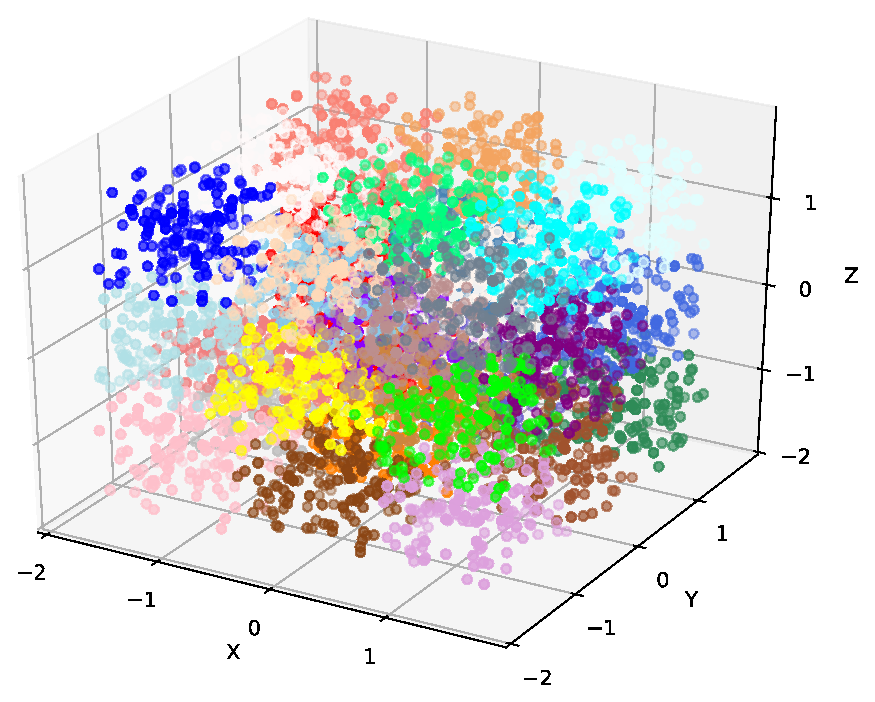
\includegraphics[width=0.85\textwidth]{fig/fig_step_32_6_150.eps}
    \caption{32 files classification.}
    \label{fig:32files}
  \end{subfigure}
  \caption{Temporal-aware sequence classification. The addresses are mapped into dots at a 3-dimensional linear space. Addresses from different files are distinguished by color.}
  \label{fig:files}
\end{figure*}

In Figure~\ref{fig:files}, we demonstrate the effectiveness of our TAC algorithm in classifying the entangled I/O workloads.
We collect the I/O trace under a dedicated multi-thread workload.
We then label all I/O request with the corresponding file id.
TAC is an unsupervised classification algorithm that classify the I/O address
in a way that the address belonging to one file is in the same cluster and vice versa.
Without loss of generality, we only show 8 files and 32 files classification in 3-dimensional linear space respectively.
However, when the number of files grows, the classification results will follow the same principles.
Obviously, as the attractive and repulsive force move the dots, the addresses from the same file gradually form clusters,
and addresses from different files are effectively separated.

\begin{figure}
\centering
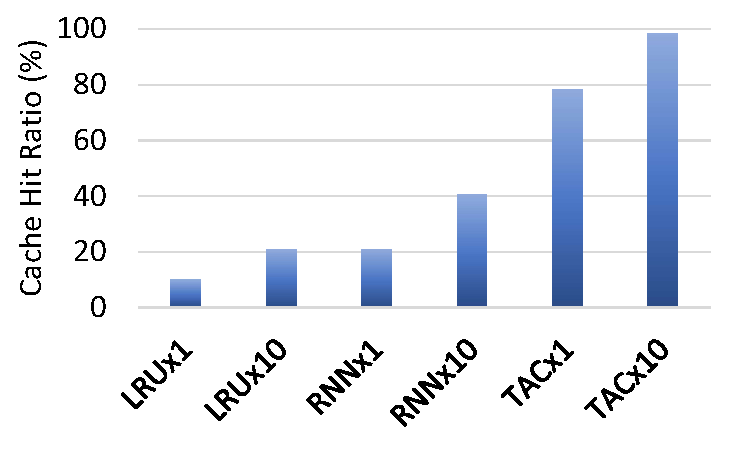
\includegraphics[width=0.45\textwidth]{fig/cache.eps}
\caption{Average cache hit ratio.}
\label{fig:cache}
\end{figure}

By using the TAC, we split the workloads into multiple clean I/O streams.
We then use the RNN model to predict the future I/Os.
We split the collected I/O trace into training and testing datasets.
We use the trained models to do the I/O prefetch and study the cache hit ratio,
and compare the performance of the traditional LRU cache,
the default LSTM (RNN) prefetcher, and the TAC + LSTM (TAC) prefetcher.
Figure~\ref{fig:cache} shows the cache hit ratio using different configurations.
We use $10^4$ files and use $0.1\%$ (in x1) and $1\%$ (in x10) respectively.
RNNx1 prefetch the first candidate predicted by the RNN model.
RNNx10 prefetch the top 10 candidates predicted by the RNN model.
TAC is the RNN with temporal-aware classification sitting in front.
TACx1 prefetch the first candidate of the RNN prefetcher.
TACx10 prefetch the top 10 candidates of the RNN prefetcher.
LRUx1 use LRU cache and reserves the same amount of cache space as the RNNx1.
LRUx10 use LRU cache and reserves the same amount of cache space as the RNNx10.
Given new learned I/O prefetcher,
we improve the cache hit ratio by 5-6 times for modern storage architecture.